\chapter{Introducción a WEKA}
% \begin{quotation}
% 	\begin{small}
%    \textit{Siempre que enseñes, enseña a la vez a dudar lo que enseñes.}
% 	\end{small}
% 	\begin{flushright}José Ortega y Gasset.\end{flushright}
% \end{quotation}



\newpage
\section{Filtros no supervisados}
%Son filtros que no tienen en cuenta la variable marca de clase.
	

	\subsection{Normalize}

	\begin{justify}
	Realiza una normalización de todos los valores numéricos en el conjunto de datos. 
	\end{justify}

	\begin{justify}
	\textbf{Uso}

	Los valores son modificados al rango [0,1], tomando el valor 0 el dato más pequeño del conjunto y tomando el valor 1 el dato mayor del mismo, quedando el resto de valores en valores continuos dentro del rango.
	\end{justify}
	
	\begin{justify}

	\textbf{Ejemplo}

	Como se observa en la figura \ref{fig:normalize1}, se tiene un conjunto de atributos originales a los cuales se les aplicará el filtro. Una vez filtrados, se puede observar en la figura \ref{fig:normalize2} cómo estos han quedado en un rango 0-1.
	\end{justify}

	\begin{figure}[!htp]
	\centering
	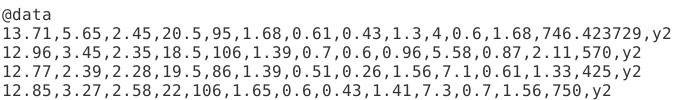
\includegraphics[scale=.32]{./figuras/image22.png}
	\caption{Base de datos 'wine'}
	\label{fig:normalize1}
	\end{figure}
	
	\begin{figure}[!htp]
	\centering
	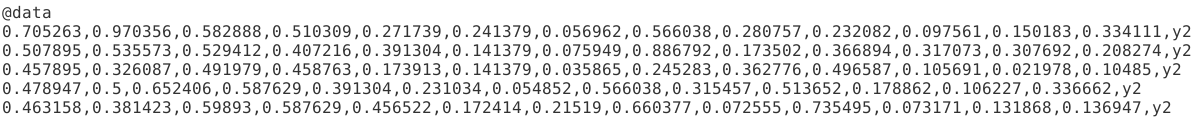
\includegraphics[scale=.32]{./figuras/image21.png}
	\caption{Base de datos 'wine' tras aplicar Normalize}
	\label{fig:normalize2}
	\end{figure}

	\subsection{ReplaceMissingValues}
	Reemplaza todo valor perdido, los cuales son representados con el signo '?', de los atributos nominales y numéricos.

	\begin{justify}
	\textbf{Uso} 
	\end{justify}

	Busca aquellos valores perdidos y los reemplaza con los valores de las modas y medias para dicho atributo.

	Para ilustrar el uso de este filtro se ha usado una pequeña base de datos que contiene notas de 3 asignaturas para varias instancias que son los alumnos, y se observa como los datos perdidos son reemplazados.

	
	\begin{justify}
	\textbf{Ejemplo}
	\end{justify}

	\begin{figure}[!htp]

	\centering
	  \subfloat[Base de datos 'notas' con valores perdidos]{
		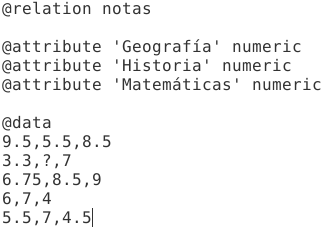
\includegraphics[scale=.32]{./figuras/image19.png}}
	  \subfloat[Media tras aplicar el filtro]{
		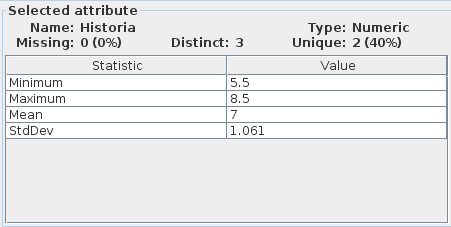
\includegraphics[scale=.32]{./figuras/image10.png}}
	\caption{Base de datos y media calculada tras aplicar ReplaceMissingValues}
	\end{figure}
  
	\begin{figure}[!htp]
	\centering
	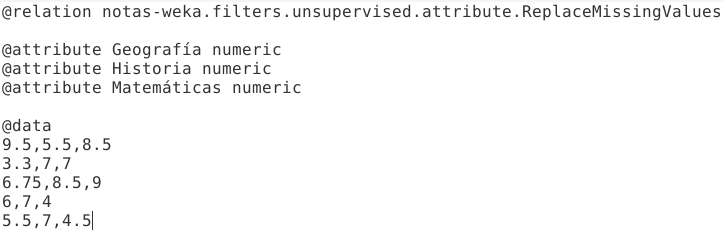
\includegraphics[scale=.32]{./figuras/image31.png}
	\caption{Fichero final con el valor perdido reemplazado}
	\end{figure}

\newpage
\subsection{RemoveUseless}
	\begin{justify}
		Elimina atributos nominales donde la varianza es muy grande o muy pequeña y que por tanto, no tienen utilidad.
	\end{justify}



	\begin{justify}
	\textbf{Uso} 
	\end{justify}
	Realiza el análisis y transformación de los componentes principales de los datos. Se usa junto con una búsqueda de Ranker. La reducción de la dimensionalidad se logra eligiendo suficientes vectores propios para tener en cuenta algún porcentaje de la varianza en los datos originales, por defecto 0.95.

	\begin{justify}
	\textbf{Ejemplo}
	\end{justify}
	Parar ilustrar este filtro se ha usado una pequeña base de datos que contiene un atributo nominal que representa un color, y 2 atributos numéricos que representan otros datos asociados. Se puede observar como el atributo nominal tiene un valor distinto para cada instancia, y por tanto, la varianza es la máxima, así pues el filtro actúa descartando dicho atributo nominal.
  

	\begin{figure}[!htp]
	\centering
	  \subfloat[Base de datos 'colores' con atributo nominal]{
		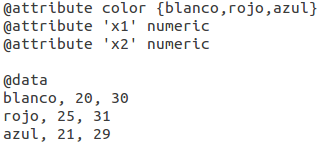
\includegraphics[scale=.45]{./figuras/image2.png}}
	  \subfloat[Fichero tras aplicar filtro]{
		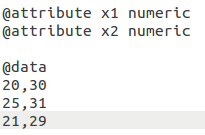
\includegraphics[scale=.5]{./figuras/image40.png}}
	\caption{Antes y después de aplicar RemoveUseless}
	\end{figure}




\newpage

	\subsection{PrincipalComponents}

	Realiza el análisis y transformación de las componentes principales de los datos.


	\begin{justify}
	\textbf{Uso} 
	\end{justify}

	La reducción de la dimensionalidad se logra eligiendo suficientes vectores propios para tener en cuenta algún porcentaje de la varianza en los datos originales (por defecto 0.95). El ruido de los atributos puede filtrarse transformándolo en el espacio de la Componente Principal, eliminando algunos de los vectores propios peores, y luego transformando de nuevo al espacio original.

	\begin{justify}
	\textbf{Ejemplo}
	\end{justify}

	
	\begin{figure}[!htp]
	\centering
	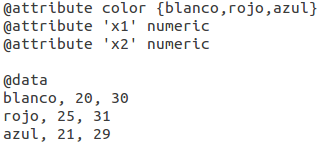
\includegraphics[scale=.42]{./figuras/image2.png}
	\caption{Base de datos 'colores'}
	\end{figure}
	
	\begin{figure}[!htp]
	\centering
	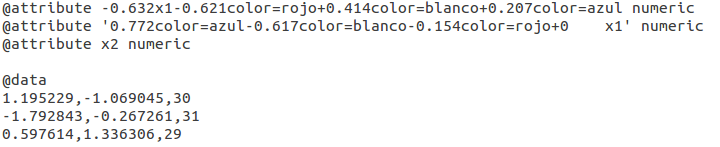
\includegraphics[scale=.42]{./figuras/image12.png}
	\caption{Fichero final tras aplicar PrincipalComponents}
	\end{figure}


\newpage

	\subsection{RandomProjection}
		Reduce la dimensionalidad de los datos proyectándolos en un subespacio de menor dimensión usando una matriz aleatoria con columnas de longitud unitaria.
	

	\begin{justify}
	\textbf{Uso} 
	\end{justify}
	
		Primero aplica el filtro NominalToBinary para convertir todos los atributos a numérico antes de reducir la dimensión. Conserva el atributo de marca de clase.

	\begin{justify}
	\textbf{Ejemplo}
	\end{justify}

		Como se muestra en la Figura 1.8 partimos de una base de datos con un atributo nominal de 3 posibles opciones 'Blanco', 'Rojo' y 'Azul' junto con un atributo numérico x1.
		Una vez aplicado el filtro, el primer atributo queda establecido en una matriz numérica de un subespacio menor. 

	\begin{figure}[!htp]
	\centering
	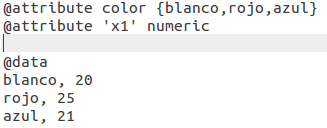
\includegraphics[scale=.42]{./figuras/image11.png}
	\caption{Base de datos 'colores' con un atributo numérico}
	\end{figure}
	
	\begin{figure}[!htp]
	\centering
	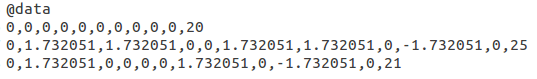
\includegraphics[scale=.42]{./figuras/image44.png}
	\caption{Fichero final tras aplicar RandomProjection}
	\end{figure}


\newpage
	\subsection{NominalToBinary}
	Convierte todos los atributos nominales en atributos binarios numéricos. 	

	\begin{justify}
	\textbf{Uso} 
	\end{justify}
	
	Un atributo con k posibles valores se transforma en k atributos binarios (0-1) si la clase es nominal. Los atributos binarios se dejan binarios. Si la clase es numérica, es posible que desee utilizar la versión supervisada de este filtro.

	\begin{justify}
	\textbf{Ejemplo}
	\end{justify}






\newpage
	\subsection{RemoveMissclassified}
	\begin{justify}
	Elimina aquellas instancias que han sido incorrectamente clasificadas, de modo que no existan valores atípicos.
	\end{justify}
	\begin{itemize}
		\item \textbf{Uso}
	\begin{justify}
	Permite escoger la marca de clase en la que se basan las clasificaciones erróneas, el clasificador 	sobre el que se basarán las clasificaciones erróneas, si el resultado será descartartado o aceptado, número de iteraciones, pliegues y umbral de error permisible.
	\end{justify}
		\item \textbf{Ejemplo}
	\end{itemize}

	\subsection{RemovePercentage}
	\begin{justify}
	Permite eliminar un porcentaje de la información de la base de datos.
	\end{justify}
	\begin{itemize}
		\item \textbf{Uso}
	\begin{justify}

	\end{justify}
		\item \textbf{Ejemplo}
	\end{itemize}

	\subsection{Resample}
	\begin{justify}
	Produce una submuestra aleatoria de un conjunto de datos utilizando el muestreo con reemplazo o sin reemplazo. 
	\end{justify}
	\begin{itemize}
		\item \textbf{Uso}
	\begin{justify}
	Se puede especificar el número de instancias en el conjunto de datos generado. Cuando se utilizan en modo por lotes, los lotes posteriores no son remuestrados.
	\end{justify}
		\item \textbf{Ejemplo}
	\end{itemize}

\newpage
\section{Filtros supervisados}
	%Son filtros que tienen en cuenta la variable marca de clase.	
	\subsection{AttributeSelection}
	\begin{justify}

	\end{justify}
	\begin{itemize}
		\item \textbf{Uso}
	\begin{justify}

	\end{justify}
		\item \textbf{Ejemplo}
	\end{itemize}
	
	\subsection{Discretize}
	\begin{justify}

	\end{justify}
	\begin{itemize}
		\item \textbf{Uso} 
	\begin{justify}

	\end{justify}
		\item \textbf{Ejemplo}
	\end{itemize}
 	
	\subsection{NominalToBinary}
	\begin{justify}

	\end{justify}
	\begin{itemize}
		\item \textbf{Uso}
	\begin{justify}

	\end{justify}
		\item \textbf{Ejemplo}
	\end{itemize}
	
	\subsection{SpreadToBinary}
	\begin{justify}

	\end{justify}
	\begin{itemize}
		\item \textbf{Uso}
	\begin{justify}

	\end{justify}
		\item \textbf{Ejemplo}
	\end{itemize}
 	
	
	\subsection{ClassBalancer}
	\begin{justify}

	\end{justify}
	\begin{itemize}
		\item \textbf{Uso}
	\begin{justify}

	\end{justify}
		\item \textbf{Ejemplo}
	\end{itemize}

	\subsection{Resampler}
	\begin{justify}

	\end{justify}
	\begin{itemize}
		\item \textbf{Uso}
	\begin{justify}

	\end{justify}
		\item \textbf{Ejemplo}
	\end{itemize}


\newpage
\section{Base de datos Wine}
	%\noindent Los objetivos principales que se persiguen en esta tesis doctoral son los siguientes:
 	
	\subsection{Detalles de la base de datos}
	
	\subsection{Modificación del fichero con nombres de atributo descriptivos}

	\subsection{Descripción de atributos y clases}

	\subsection{Tratamiento de elementos perdidos}

	\subsection{Diferencia entre Distinct y Unique}

	\subsection{Eliminar atributos identificadores}
	
	\subsection{Relaciones visualmente significativas en entorno Visualice}
	

\newpage
\section{Aplicación de 6 filtros a la base de datos}
	%\noindent Los objetivos principales que se persiguen en esta tesis doctoral son los siguientes:
 	
	\subsection{Filtro de selección de características}
	\begin{itemize}
		\item \textbf{Uso}
		\item Resultados:
		\item \textbf{Ejemplo}
	\end{itemize}

	\subsection{Filtro de selección de patrones}
	\begin{itemize}
		\item \textbf{Uso}
		\item Resultados:
		\item \textbf{Ejemplo}
	\end{itemize}

	\subsection{Filtro de filters/supervised/attribute/*}
	\begin{itemize}
		\item \textbf{Uso}
		\item Resultados:
		\item \textbf{Ejemplo}
	\end{itemize}

	\subsection{Filtro de filters/supervised/instance/*}
	\begin{itemize}
		\item \textbf{Uso}
		\item Resultados:
		\item \textbf{Ejemplo}
	\end{itemize}

	\subsection{Filtro de filters/unsupervised/attribute/*}
	\begin{itemize}
		\item \textbf{Uso}
		\item Resultados:
		\item \textbf{Ejemplo}
	\end{itemize}

	\subsection{Filtro de filters/unsupervised/instance/*}
	\begin{itemize}
		\item \textbf{Uso}
		\item Resultados:
		\item \textbf{Ejemplo}
	\end{itemize}



\newpage
\section{Conversión de todo atributo nominal a codificación binaria}


\newpage
\section{División de la base de datos en particiones}

	\subsection{División en 10-Holdout 75-25}
	\begin{itemize}
		\item \textbf{Uso}
		\item Resultados:
		\item \textbf{Ejemplo}
	\end{itemize}


	\subsection{División en 10-Fold}
	\begin{itemize}
		\item \textbf{Uso}
		\item Resultados:
		\item \textbf{Ejemplo}
	\end{itemize}

% 	A continuación y una vez descritos los objetivos de esta tesis doctoral, se exponen
% 	las aportaciones fundamentales incluidas en esta memoria:
% 	\begin{enumerate}
% 	\item Análisis y descripción de los aspectos más importantes en el uso de algoritmos
% 	evolutivos mono-objetivo y multi-objetivo híbridos, funciones de aptitud, DE y
% ensembles para el diseño de modelos de red para clasificación de
% 	patrones.
% 	\item Implementación de varias versiones de un AE memético mono-objetivo usando
% 	modelos de red puros e híbridos en capa oculta. Los resultados obtenidos están en
% 	consonancia con los	de otras	técnicas	frecuentemente citadas en Aprendizaje
% Automático (\textit{Machine Learning}, ML).
% 	\item Implementación de un MOEA	memético basado en dominancia de Pareto para diseñar
% 	modelos de	red para clasificación	de patrones.
% 	\item Implementación de varias versiones de un MOEA memético basado
% 	en dominancia de	Pareto y en la DE.
% 	\item Futura obtención de	padres virtuales en DE basados en
% 	los valores extremos y mejores individuos de la 	población.
% 	\item Estudio y análisis del uso de la mínima sensibilidad en la	clasificación de
% 	patrones	para problemas multiclase, como alternativa al uso de	curvas ROC y otras
% 	medidas
% 	de	rendimiento. Utilización de dicha función de aptitud en los algoritmos
% 	desarrollados obteniéndose resultados satisfactorios.
% 	\item Nueva representación en dos dimensiones de la bondad de un clasificador
% 	mediante la optimización simultánea de la precisión y la mínima sensibilidad.
% 	\item Aplicación de los algoritmos implementados en la resolución de problemas de
% 	clasificación reales de microbiología predictiva, teledetección y predicción de viento.
% % 	\item Inclusión los algoritmos implementados en KEEL,
% % 	ampliando de esta manera el abanico de técnicas de las que dispone la herramienta,
% % 	proporcionándole una mayor riqueza para labores científicas.
% 	\end{enumerate}
